\documentclass{beamer}
\mode<presentation>

\usepackage{beamerthemesplit}
\usepackage[francais]{babel}
\usepackage[utf8x]{inputenc}
\usepackage[T1]{fontenc}
\usepackage{graphicx}
\usepackage{eurosym}
\usepackage{listings}
\usepackage{hyperref}
\usepackage{xcolor}

% Gconfs is Orange !
\definecolor{gris}{HTML}{606060}
\definecolor{gris-clair}{rgb}{0.9,0.9,0.9}
\definecolor{orange}{rgb}{1,0.5,0.25}

\definecolor{lightgray}{RGB}{240,240,240}

\definecolor{vert}{RGB}{0,176,80}
\definecolor{verta}{RGB}{79,97,40}
\definecolor{vertb}{RGB}{195,214,155}
\definecolor{vertc}{RGB}{235,241,221}
\definecolor{bleua}{RGB}{31,73,125}
\definecolor{bleub}{RGB}{219,229,241}
\definecolor{rougea}{RGB}{192,80,77}
\definecolor{rougeb}{RGB}{242,220,219}
\definecolor{orangea}{RGB}{233,132,45}
\definecolor{orangeb}{RGB}{188,84,7}

\definecolor{brown}{RGB}{128,0,0}
\definecolor{blue}{RGB}{0,0,255}
\definecolor{green}{RGB}{0,128,0}
\definecolor{seagreen}{RGB}{69,158,181}

\usetheme{Darmstadt} %%% Thème que j'ai choisi pour les slides

\setbeamercovered{transparent}
\setbeamercolor{structure}{bg=black,fg=orangea}

% EOGT End Of Gconfs Theme

\title{Choisir son clavier}
\author[PM \and Colona]{
  Pierre-Marie \textsc{de Rodat} (PM, \texttt{de-rod\_p})\\
  \and Ivan \textsc{Delalande} (Colona, \texttt{delala\_i})
}
\date{\today}

\begin{document}

\begin{frame}
    \begin{center}
        
\includegraphics[scale=0.35]{images/gconfs.png}
    \end{center}
    \maketitle
\end{frame}

\section*{Introduction}

\begin{frame}{Mais pourquoi~?}
  \begin{itemize}
    \item Difficultés avec les QWERTY sur les postes du campus IONIS~: \pause
      \begin{itemize}
        \item Rapidité \pause
        \item Précision \pause
        \item Jeu de caractères
      \end{itemize}\pause

    \item Le clavier est très utilisé~: important de mieux faire \pause
      \begin{itemize}
        \item Chez soi, en examen et partout ailleurs~! \pause
        \item Changement si possible avant la première année d’ingénieur~!
      \end{itemize}\pause
	\item Vos mains sont précieuses, chérissez-les~!
  \end{itemize}
\end{frame}


%\AtBeginSection{
%  \begin{frame}
%    \tableofcontents[currentsection]
%  \end{frame}
%}

\section{Vocabulaire}

\begin{frame}{Clavier et keymap}
  \begin{itemize}
    \item Clavier~: dispositif \emph{physique} permettant la saisie. Exemple~: les différents modèles du PIE, le TypeMatrix. \pause
    \item Keymap~: utilisation \emph{logique} du clavier par le système. Exemple~: les dispositions QWERTY, QWERTZ, AZERTY, Dvorak US,  Bépo
  \end{itemize}
\end{frame}



\subsection{Clavier}

\begin{frame}{Anatomie d’un clavier}
  \begin{itemize}
    \item Ensemble de touches disposées sur une «~planche~» \pause
    \item Plusieurs groupes~: pavé alphanumérique, directionnel, numérique, touches de fonction, … \pause
    \item Plusieurs dispositions écrites \pause
    \item Plusieurs paramètres ergonomiques~: taille, éloignement, disposition, profondeur, résistance
  \end{itemize}
\end{frame}

\begin{frame}{Les claviers aujourd’hui}
  \begin{itemize}
    \item Pavé alphanumérique, directionnel, numérique, touches de fonctions (parfois touches multimédia) \pause
    \item Rangées du pavé alphanumérique décalées en escalier («~clavier droit~») \pause
    \item Touches «~Backspace~» et «~Enter~» peu accessibles \pause
  \end{itemize}

  Il existe des alternatives (rarement utilisées)~: \pause
  \begin{itemize}
    \item Claviers compacts~: suppression de pavés (souvent le pavé numérique) \pause
    \item Touches en matrice \pause
    \item «~Backspace~» et «~Enter~» au milieu du pavé alphanumérique
  \end{itemize}
\end{frame}



\subsection{Keymap}

\begin{frame}{Caractéristiques d’une keymap}
  \begin{itemize}
    \item
  \end{itemize}
\end{frame}

\begin{frame}{Les keymaps aujourd’hui}
  \begin{itemize}
    \item De trop nombreuses dispositions existent: colemak, svorak, dvorak(gaucher, droiter, international), bepo, bepo-fr, qwerty, azerty, ...
  \end{itemize}
\end{frame}

\section{Le matériel}

\subsection{Intérêt}
\begin{frame}{Pourquoi existe-t-il des clavier de 5~à~500€~?}
    \begin{itemize}
        \item Les claviers standards héritent des lourdeurs du passé: touches
        en diagonale, position  du retour à la ligne, du backspace, … \pause
        \item Il existe des claviers ergonomiques, bien plus pratiques (touches
        mécaniques, clavier matriciel, …).
    \end{itemize}
\end{frame}

\subsection{Exemples}
\begin{frame}{Exemples — Typematrix}
  \begin{figure}
    \centering
    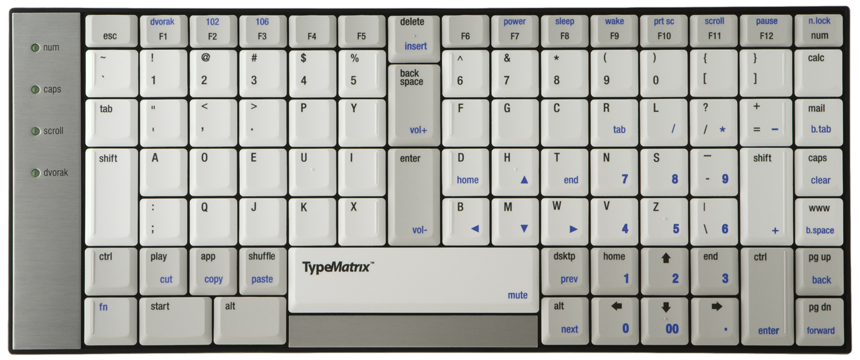
\includegraphics[height=100pt]{images/2030-dvorak.png}
  \end{figure}
\end{frame}

\begin{frame}{Exemples — Truly-Ergonomics}
  \begin{figure}
    \centering
    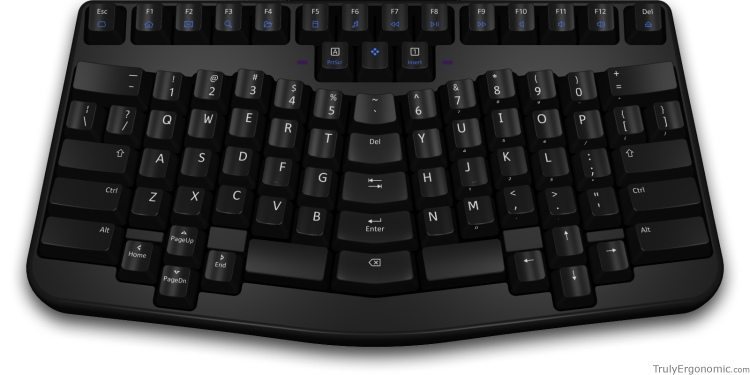
\includegraphics[height=100pt]{images/t_e_keyboard.jpg}
  \end{figure}

  Et d’autres encore~: Kinesis, Maltron\dots
\end{frame}

\section{Keymaps alternatives}

% Troll disclaimer~: on ne s’intéresse qu’aux keymaps qui peuvent intéresser la
% majorité des épitéens…

\begin{frame}{Généralités}
    \begin{itemize}
        \item «~X n’est pas adapté au code, c’est plus facile en QWERTY~» \pause
            \begin{itemize}
                \item Les avis divergent fortement, faites-vous votre propre
                  avis. \pause

                \item Le code est généralement composé de mots anglais, plus
                  des commentaires.
            \end{itemize}
            \pause

        \item Keymap adaptée au français~: toujours plus adaptée à
          l’anglais qu’un QWERTY ou AZERTY
          % Ce sont deux langues d’origine plus ou moins latines, assez
          % similaires.
    \end{itemize}
\end{frame}



\subsection{Canadien multiligue}

\begin{frame}{Canadien multilingue}
    \centering
    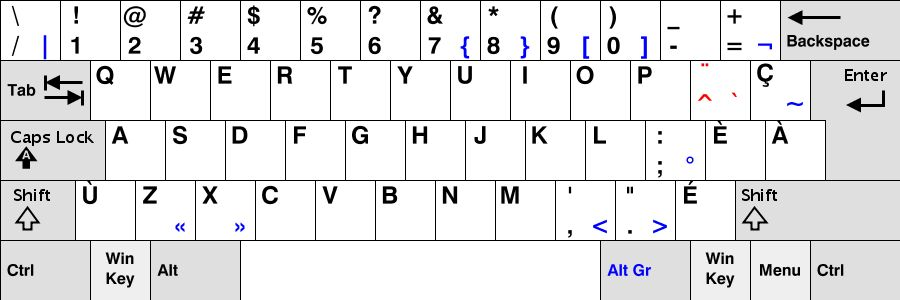
\includegraphics[width=\textwidth]{images/ca-multi.jpg}
    \pause

    \begin{itemize}
        \item Très proche du QWERTY \pause

        \item Accès direct à la plupart des signes typographiques français
          courants (il en manque certains comme «~…~») \pause
        % Lettres accentuées (et «~ç~») en accès direct, ainsi que les
        % majuscules avec Shift, espace insécable

        \item Accès direct aux chiffres (pas besoin de Shift) \pause

        \item Délimiteurs par paire («~[~» à côté de «~]~», idem pour «~(~»,
          etc.)
    \end{itemize}
\end{frame}



\subsection{US International}

\begin{frame}{US International}
    \centering
    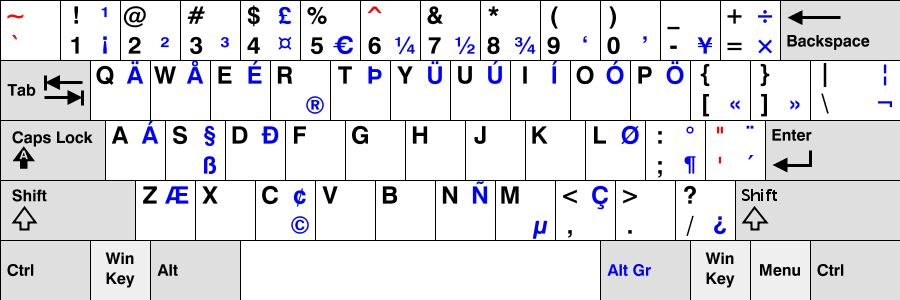
\includegraphics[width=\textwidth]{images/us-intl.jpg}
    \pause

    \begin{itemize}
	\item Quasiment identique au QWERTY \pause

        \item Rajout de quelques caractères supplémentaires (accès~: touches mortes ou Alt~Gr)
    \end{itemize}
\end{frame}



\subsection{Dvorak — DSK}

\begin{frame}{Le Dvorak}
    \centering
    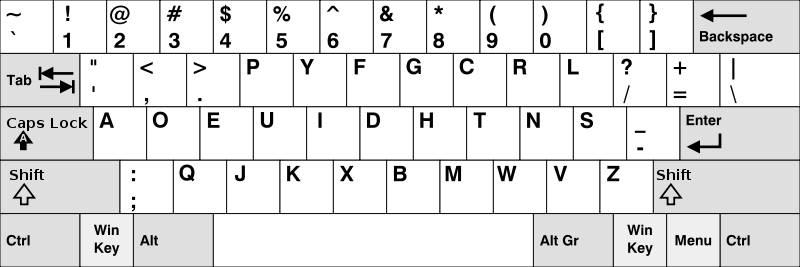
\includegraphics[height=90pt]{images/dvorak.png}
    \pause

    \begin{itemize}
	\item Le dvorak, ou clavier américain simplifié (DSK). \pause

	\item Conçu par la méthode Dvorak~: en étudiant les langues
          cibles. \pause

	\item Créé dans les années 1930 par August Dvorak et William Dealey.
    \end{itemize}
\end{frame}

\begin{frame}{Le DSK}
    \begin{itemize}
	\item Clavier inadaptable pour d’autre langues. \pause

	\item Quelques unes pour le français (Dvorak-fr, fr-Dvorak,
          Dvorak-international). \pause

	\item Une seule tient la route~: le Bépo.
    \end{itemize}
\end{frame}



\subsection{Bépo}

\begin{frame}{Caractéristiques}
    % Ne pas oublier de parler de la création du Bépo (communauté sur Internet,
    % méthode Dvorak et donc étude statistique, améliorations successives, et
    % version maintenant stable)

    \centering
    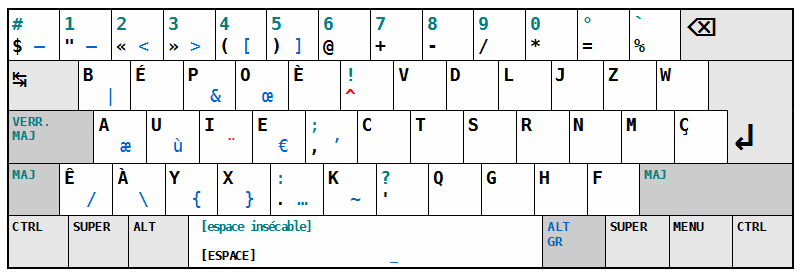
\includegraphics[width=\textwidth]{images/bepo-simple.png}
    \pause

    \begin{itemize}
	\item 70~\% des lettres nécessaires sont sur la ligne centrale~: moins
          de mouvement pour les mains. \pause

        \item Disposition telle qu’il y ait le plus d’alternance possible entre
          les deux mains. \pause

	\item S’apprend très facilement.
    \end{itemize}
\end{frame}

\begin{frame}{Carte complète}
    \centering
    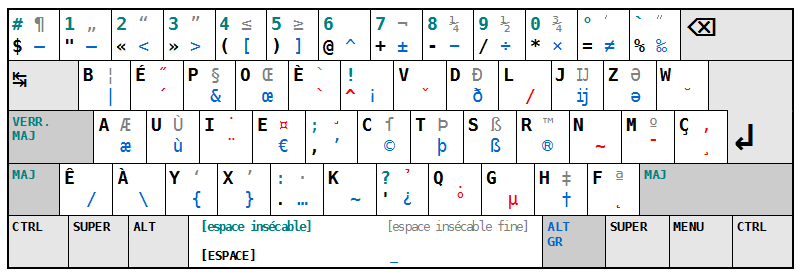
\includegraphics[width=\textwidth]{images/bepo-complete.png}
    \pause

    \begin{itemize}
        \item Le jeu de caractères facilement accessible est \emph{très}
          riche. \pause

        \item Il est particulièrement adapté au français~: lettres et signes
          typographiques.
    \end{itemize}
\end{frame}

\section{Utilisation}



\subsection{Bon usage d’un clavier}

\begin{frame}{Bon usage d’un clavier}
    Objectifs~:
    \begin{itemize}
        \item Saisir rapidement et avec précision \pause

        \item Avoir une posture confortable et saine
    \end{itemize}
    \pause

    Moyens~:
    \begin{itemize}
        \item Bien positionner son clavier par rapport à soi \pause

        \item Bien positionner ses doigts sur les touches au repos \pause

        \item Pour chaque touche, utiliser le doigt associé \pause

        \item Ne pas jongler entre écran et clavier (donc ne pas regarder le clavier)
    \end{itemize}
\end{frame}



\subsection{Apprentissage}

\begin{frame}{Les utilitaires}
    \begin{itemize}
        \item But~: parvenir à maîtriser une keymap ou un clavier le plus
          rapidement-efficacement possible \pause
        \item Demande un peu d’exercice chaque jours pendant une ou deux
          semaines, un peu de pratique, et c’est gagné~! \pause

        \item GNU Typist \pause
        \item Klavaro (Windows, GNU/Linux, toute keymap) \pause
        \item Ktouch (GNU/Linux) \pause
        \item TypeTrainer4Mac (Mac OS X) \pause
	    \item Le pld Bépo (interactif) \pause
		\item The Typing of the Dead (Windows)
    \end{itemize}
\end{frame}

\begin{frame}{Conditions}
    Pour l’épitéen typique~:
    \begin{itemize}
        \item Demande un minimum de motivation (penser aux avantages) \pause

        \item \emph{À éviter pendant un rush~!!!} \pause

        \item Les vacances sont le moment idéal (pas besoin de productivité)
    \end{itemize}
\end{frame}



\subsection{Changer la keymap d’un clavier}

\begin{frame}{Microsoft Windows}
    Deux possibilités (reviennent à peu près au même)~:
    \pause
    \begin{itemize}
        \item Dans le panneau de configuration, ouvrir l’item «~Clavier~» ou
          «~Service de texte et de langues~», puis ajouter la keymap voulue et
          la mettre par défaut dans l’onglet «~Général~». \pause

        \item Ajouter la keymap voulue dans le menu de la «~Barre de langue~»
          et la sélectionner avant de l’utiliser.
    \end{itemize}
\end{frame}

\begin{frame}{Mac OS X}
    \begin{itemize}
        \item Tout se passe dans le menu «~International~» (dans les
          préférences système)~: item «~Langue et texte~», onglet «~Input~»
          \pause

        \item Il s’agit d’activer des keymaps, pour ensuite les sélectionner
          dans l’icône de la barre de menus.
    \end{itemize}
\end{frame}

\begin{frame}{GNU/Linux et *BSD}
    \begin{itemize}
        \item Pour changer la keymap de X~: \pause
            \begin{itemize}
                \item Par interface graphique~: dépend du gestionnaire de
                  bureau utilisé \pause

                \item En ligne de commande~:
                  \newline \texttt{setxkbmap us}
                  \newline \texttt{setxkbmap us intl}
                  \newline \texttt{setxkbmap ca multi}
                  \newline \texttt{setxkbmap fr}
                  \newline \texttt{setxkbmap fr bepo}
                  ...
            \end{itemize}
            \pause

        \item Pour changer la keymap des tty~: dépend fortement du système et
          de la distribution utilisés…\pause
    \end{itemize}
\end{frame}

\section*{Ressources}

\begin{frame}{Ressources}
	\begin{itemize}
		\item \url{http://geekhack.org}\\
		communauté d’amateurs de claviers,
		\item {\footnotesize
		\url{http://www.overclock.net/t/491752/mechanical-keyboard-guide}}\\
		guide sur les claviers,
	\end{itemize}
	~\\
	\begin{itemize}
		\item \url{http://en.wikipedia.org/wiki/Keymap}\\
		présentation d’un grand nombre de keymaps,
		\item \url{http://bepo.fr}\\
		site dédié à la keymap Bépo.
	\end{itemize}
\end{frame}


\end{document}
